\begin{figure}
\centering
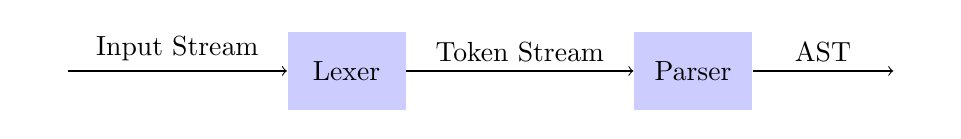
\begin{tikzpicture}[scale=2,
invisible/.style={rectangle, minimum size=5mm},
node/.style={rectangle, fill=blue!20, minimum size=15mm, minimum height=10mm}
]
\node[invisible] (westedge) at (0, 0) {};
\node[node] (lexer) at (1.9, 0) {Lexer};
\node[node] (parser) at (4.1, 0) {Parser};
\node[invisible] (eastedge) at (5.5, 0) {};

\draw[->] (westedge) -- (lexer) node[midway, above] {Input Stream};
\draw[->] (lexer) -- (parser) node[midway, above] {Token Stream};
\draw[->] (parser) -- (eastedge) node[midway, above] {AST};
\end{tikzpicture}

\caption{The flow of data within a parser.}
\label{fig:lexerparserdiagram}
    
\end{figure}